\documentclass{article}
\usepackage[utf8]{inputenc}
\title{XinFOAM}
\author{Shaohui Chen}
\usepackage{enumitem}
\usepackage[left=2.5cm,right=2.5cm,top=3cm,bottom=3cm]{geometry}
\usepackage{natbib}
\usepackage{graphicx}
\usepackage{xcolor}
\usepackage[colorlinks = true,
            linkcolor = blue,
            urlcolor  = blue,
            citecolor = blue,
            anchorcolor = blue]{hyperref}
\usepackage{pdflscape}
\usepackage{array}
\usepackage{makecell}
\renewcommand\theadalign{bc}
\renewcommand\theadfont{\bfseries}
\renewcommand\theadgape{\Gape[4pt]}
\renewcommand\cellgape{\Gape[4pt]}
\usepackage{geometry}
\usepackage{graphicx}
\usepackage{subcaption}
\usepackage{amsmath,esint}
\captionsetup{justification=raggedright,singlelinecheck=false}
\usepackage{setspace}
\renewcommand{\baselinestretch}{1.2} 
\setlength{\parskip}{0.75em}
\DeclareUnicodeCharacter{2212}{-}
\begin{document}
\maketitle
\tableofcontents
\newpage
\part{Theory background}
\section{Theory}
\subsection{Navier Stokes Equations}

The Navier Stokes describe the motion of viscous fluid substances. These balance equations are derived by applying the mass conservation and Newton's second law (momentum conservation principles) to a control volume. Additionally, energy or other interested fields. 

\subsubsection{Mass Conservation}

The mass conservation in a 2D controlled volumes (CV)is readily derived as: 

[Rate of mass change in CV] = [Rate of mass flow into CV] - [Rate of mass flow out of CV]

\begin{figure}[h!]
\centering
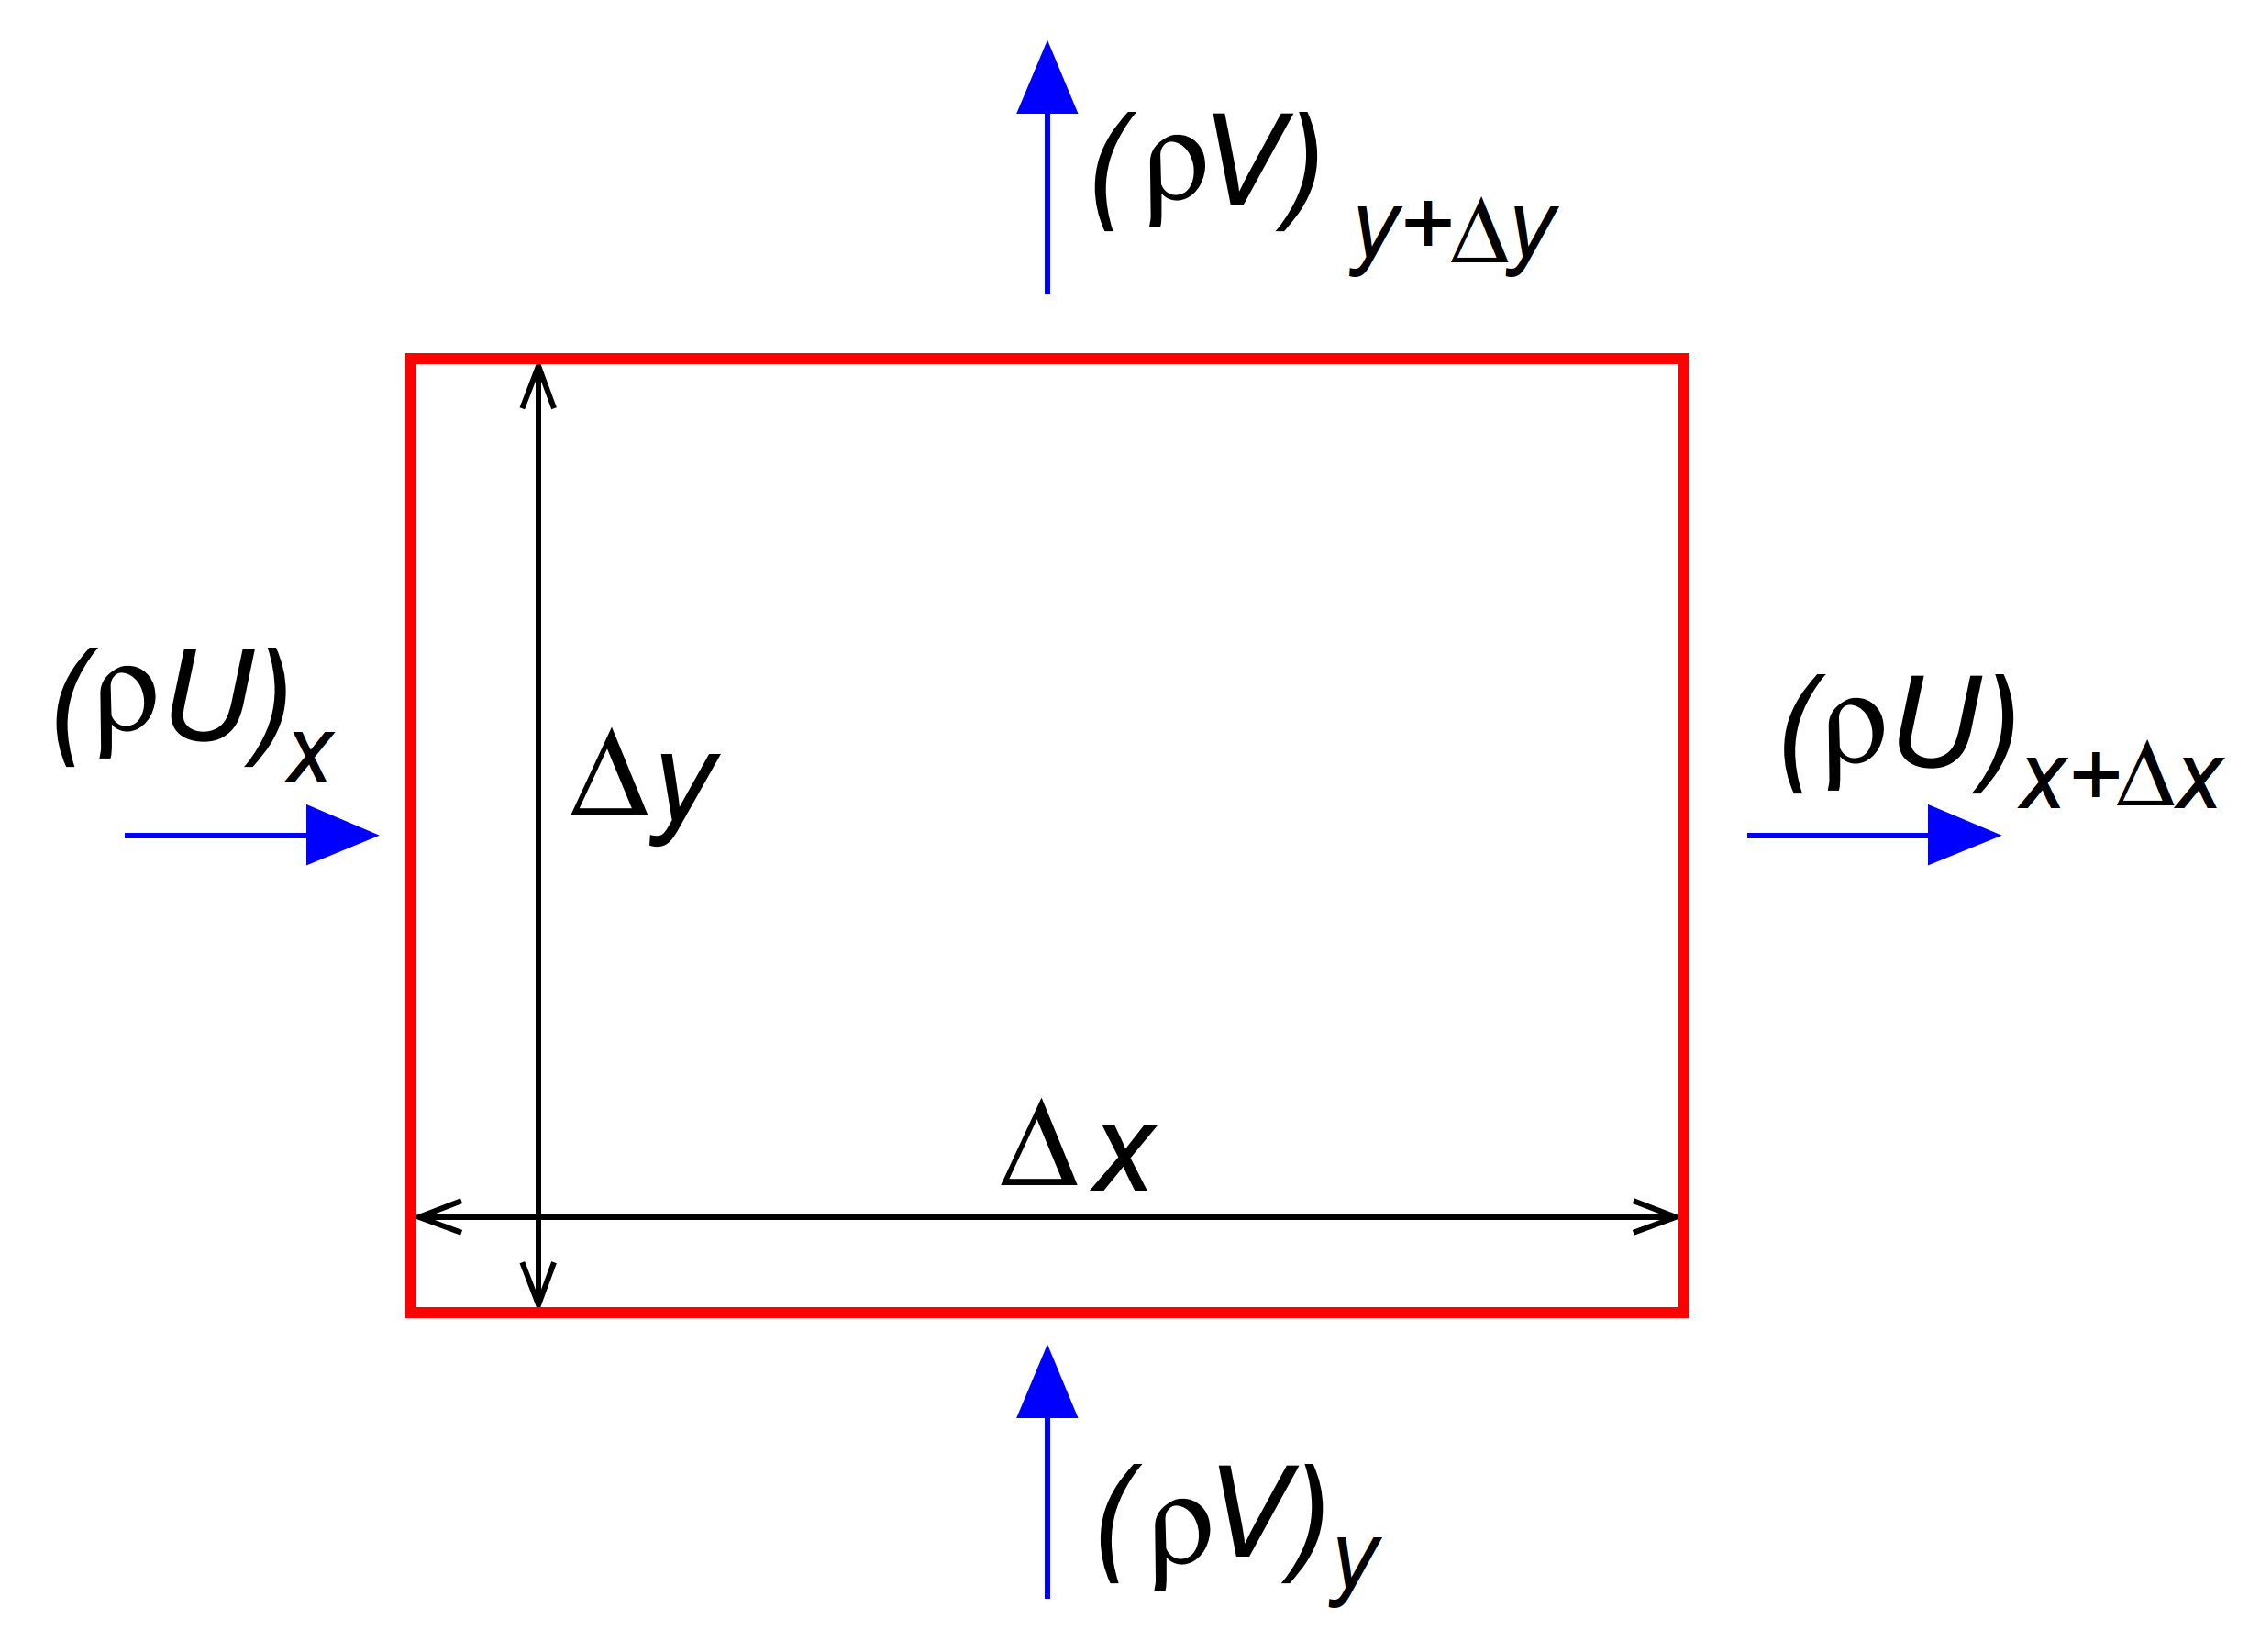
\includegraphics[scale=0.15]{ns 2D mas sketch.PNG}
\label{fig:ns 2D mas sketch.PNG}
\caption{The conservation of mass in a controlled volume}
\end{figure}

\begin{equation}
\frac{\partial (\rho\Delta x \Delta y)}{\partial t}  = (\rho U)_x \Delta y + (\rho V)_y \Delta x - \left[(\rho U)_{x+\Delta x} \Delta y + (\rho V)_{y + \Delta y} \Delta x \right]
\label{eq:mass conservation 1} 
\end{equation}

Division with $\Delta x \Delta y$ and rearrange the equation leads to:
\begin{equation}
\frac{\partial \rho}{\partial t}  = \frac{(\rho U)_x - (\rho U)_{x+\Delta x}}{\Delta x} + \frac{\Delta y - (\rho V)_{y + \Delta y}}{\Delta y} 
\label{mass conservation} 
\end{equation}

At the limit $\Delta t \rightarrow 0$, control volume shrink to infinitesimally small, using Taylor expansion: 
$$(\rho U)_{x + \Delta x} = (\rho U)_x + \Delta x \frac{\partial (\rho U)_x}{\partial x}$$. 
Devision with $\Delta x \Delta y$ and rearrange the equation leads to:
\begin{equation}
\frac{\partial \rho}{\partial t} + \frac{\partial (\rho U)}{\partial x} + \frac{\partial (\rho V)}{\partial y} + \frac{\partial (\rho W)}{\partial z} = 0 \text{ or } \frac{\partial \rho}{\partial t} + \frac{\partial (\rho u_i)}{\partial x_i} = 0
\label{eq: mass conservation 2} 
\end{equation}

\subsubsection{Momentum Conservation}

The momentum conservation principle is:
 
[Rate of momentum change in CV ] = 

[Rate of momentum flow into CV] - [Rate of momentum flow out of CV] 

+ [Force acting on CV faces] + [Body forces within CV]

\begin{figure}[h!]
\centering
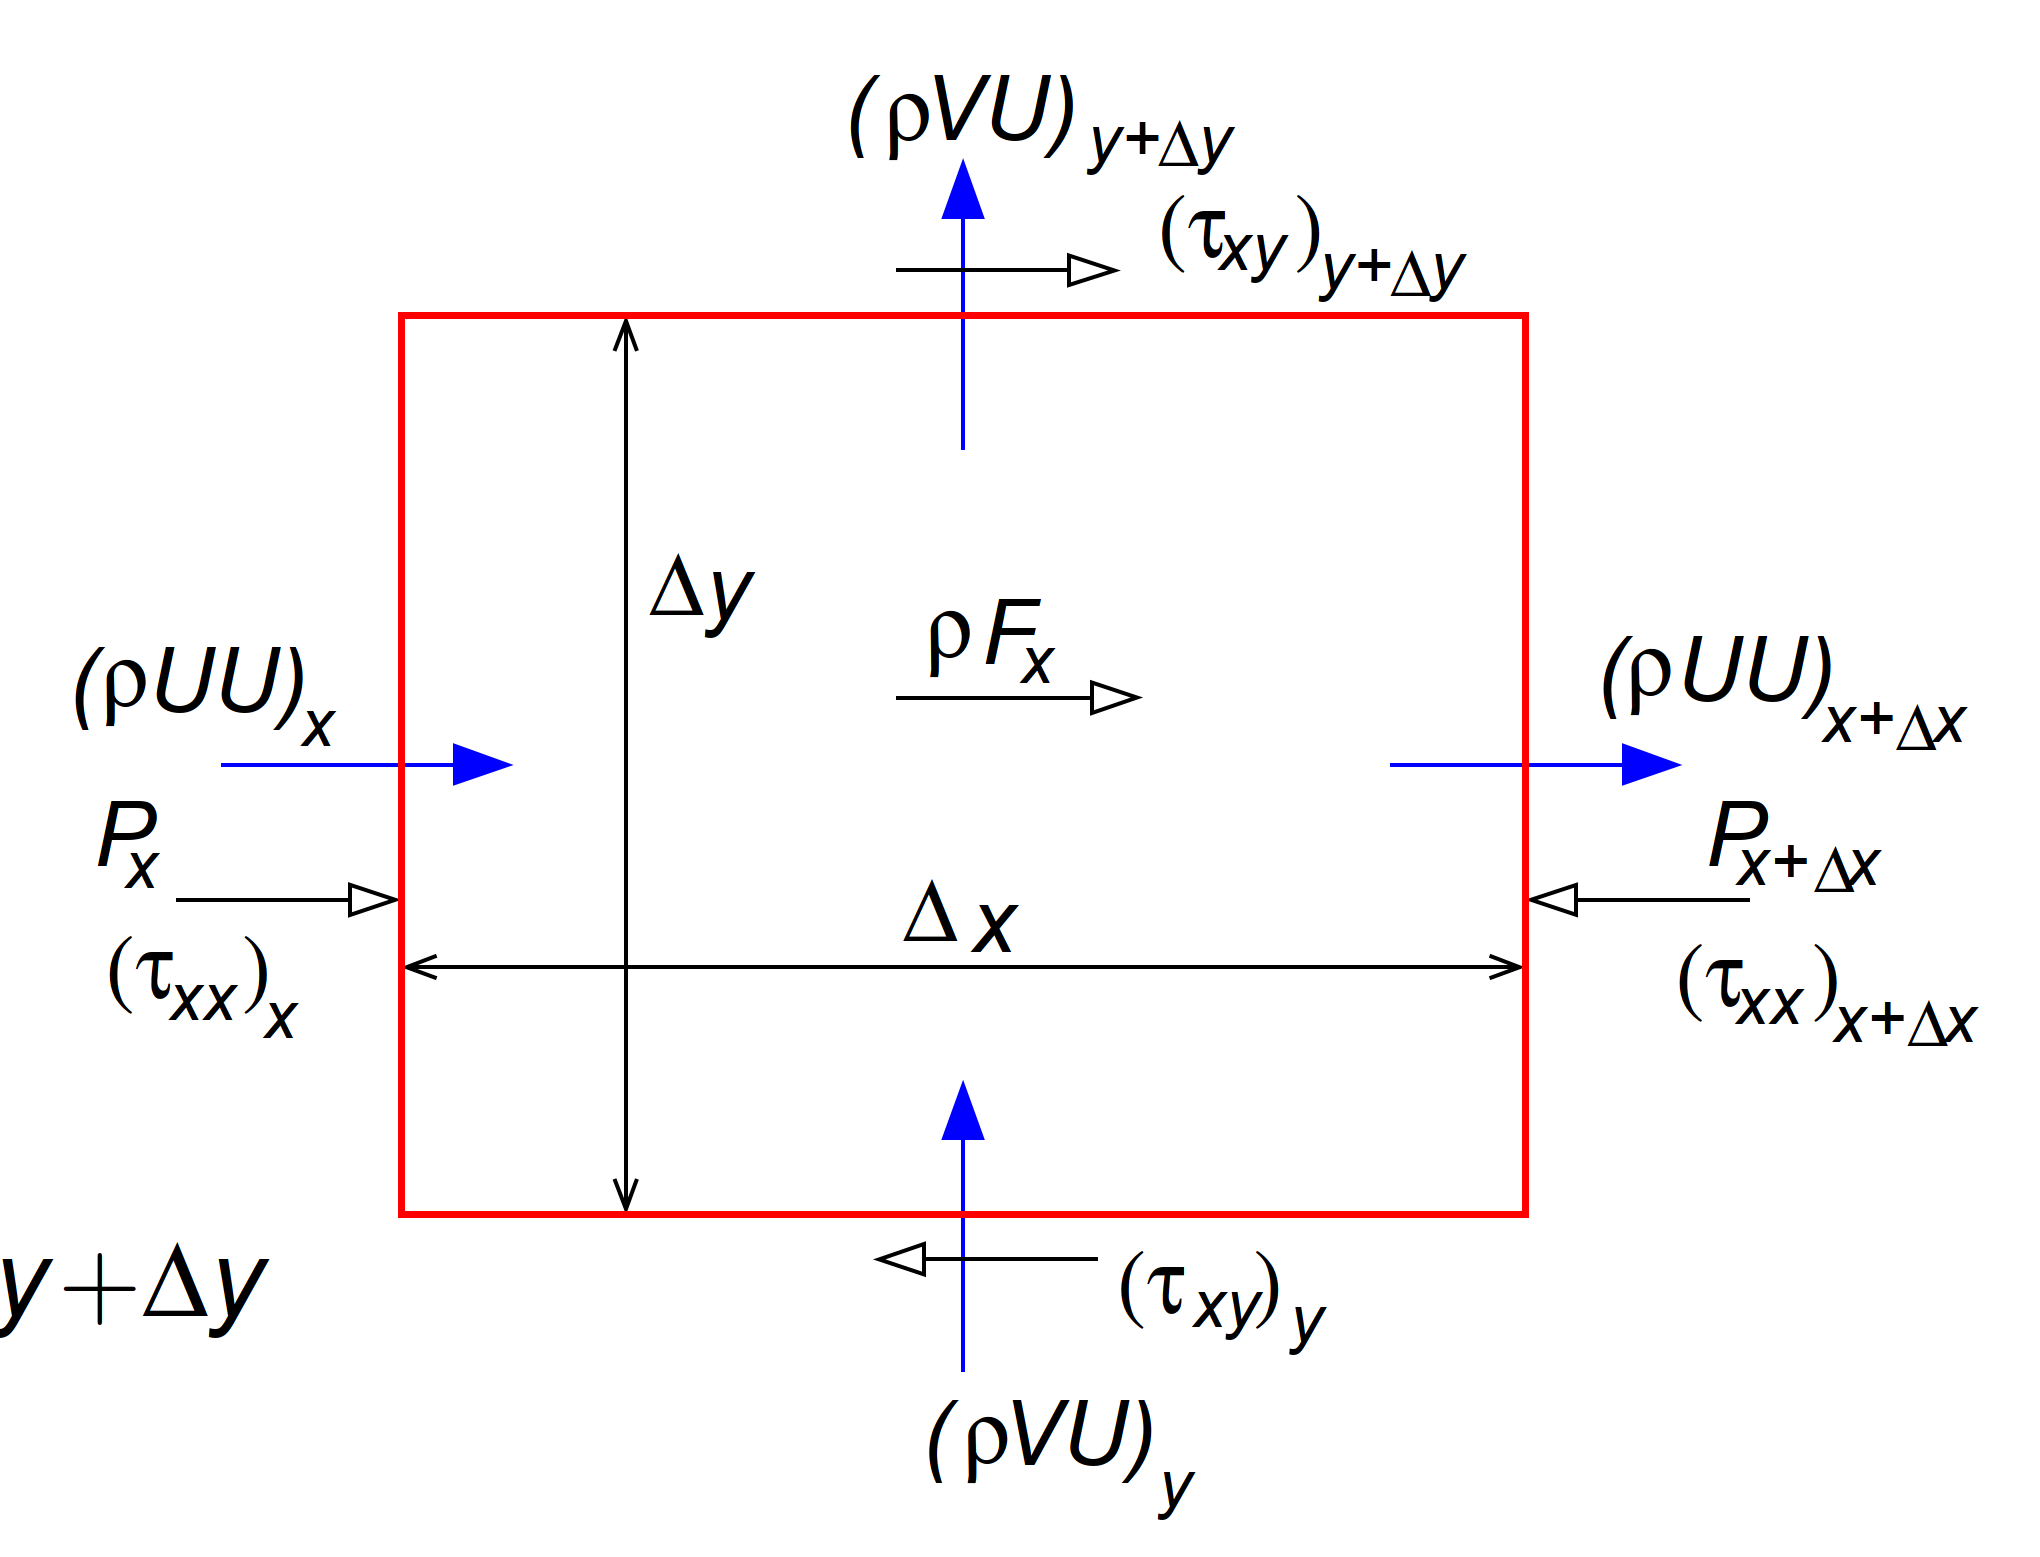
\includegraphics[scale=0.15]{ns 2D momentum sketch.PNG}
\caption{momentum on a CV}
\label{fig:ns 2D momentum sketch.PNG}
\end{figure}

In $x$ direction the momentum conservation is 
\begin{align*}
\underbrace{\Delta x \Delta y \left[\partial \left( \rho U \right) / \partial t \right]}_{\text{Momentum change Rate}} & = \underbrace{\left[((\rho U U)_x -\rho U U)_{x + \Delta x} \right]\Delta y + \left[(\rho V V)_y -(\rho V V)_{y + \Delta y} \right]\Delta x}_{\text{Momentum net flow}} \\ 
&+ \underbrace{\left[ (p + \tau_{xx})_x - (p + \tau_{x x})_{x + \Delta x}) \right]\Delta y + \left[\tau_{xy})_y -( (\tau_{xy})_{y + \Delta y}) \right] \Delta x}_{\text{Net surface force}}  \\
& + \underbrace{\rho F_x \Delta x \Delta y}_{\text{Body force}}
\end{align*}
Divide by $\Delta x \Delta y$ and at limit $\Delta x \rightarrow 0 \text{ and } \Delta y \rightarrow 0$. Expand it to 3-D. 

\begin{equation}
\frac{\partial(\rho U)}{\partial t} + \frac{\partial (\rho U^2)}{\partial x} + \frac{\partial (\rho UV)}{\partial y} +\frac{\partial (\rho UW)}{\partial z} = -\frac{\partial p}{\partial x} -\frac{\partial \tau_{xx}}{\partial x} - \frac{\partial \tau_{xy}}{\partial y} - \frac{\partial \tau_{xz}}{\partial z} + \rho F_x
\label{eq:momentum x}
\end{equation}
Similarly applies to $y$ and $z$ directions. And put it in index form: 
\begin{equation}
\frac{\partial(\rho u_i)}{\partial t} + \frac{\partial (\rho u_i u_j)}{\partial x_j} = -\frac{\partial p}{\partial x_i} - \frac{\partial \tau_{ij}}{\partial x_j} + \rho F_i
\end{equation}

The shear stress in the above equation is also related to the velocity. Consider a flat plate on the top surface moves at constant velocity $U$ while the bottom wall is fixed.
\begin{figure}[h!]
\centering
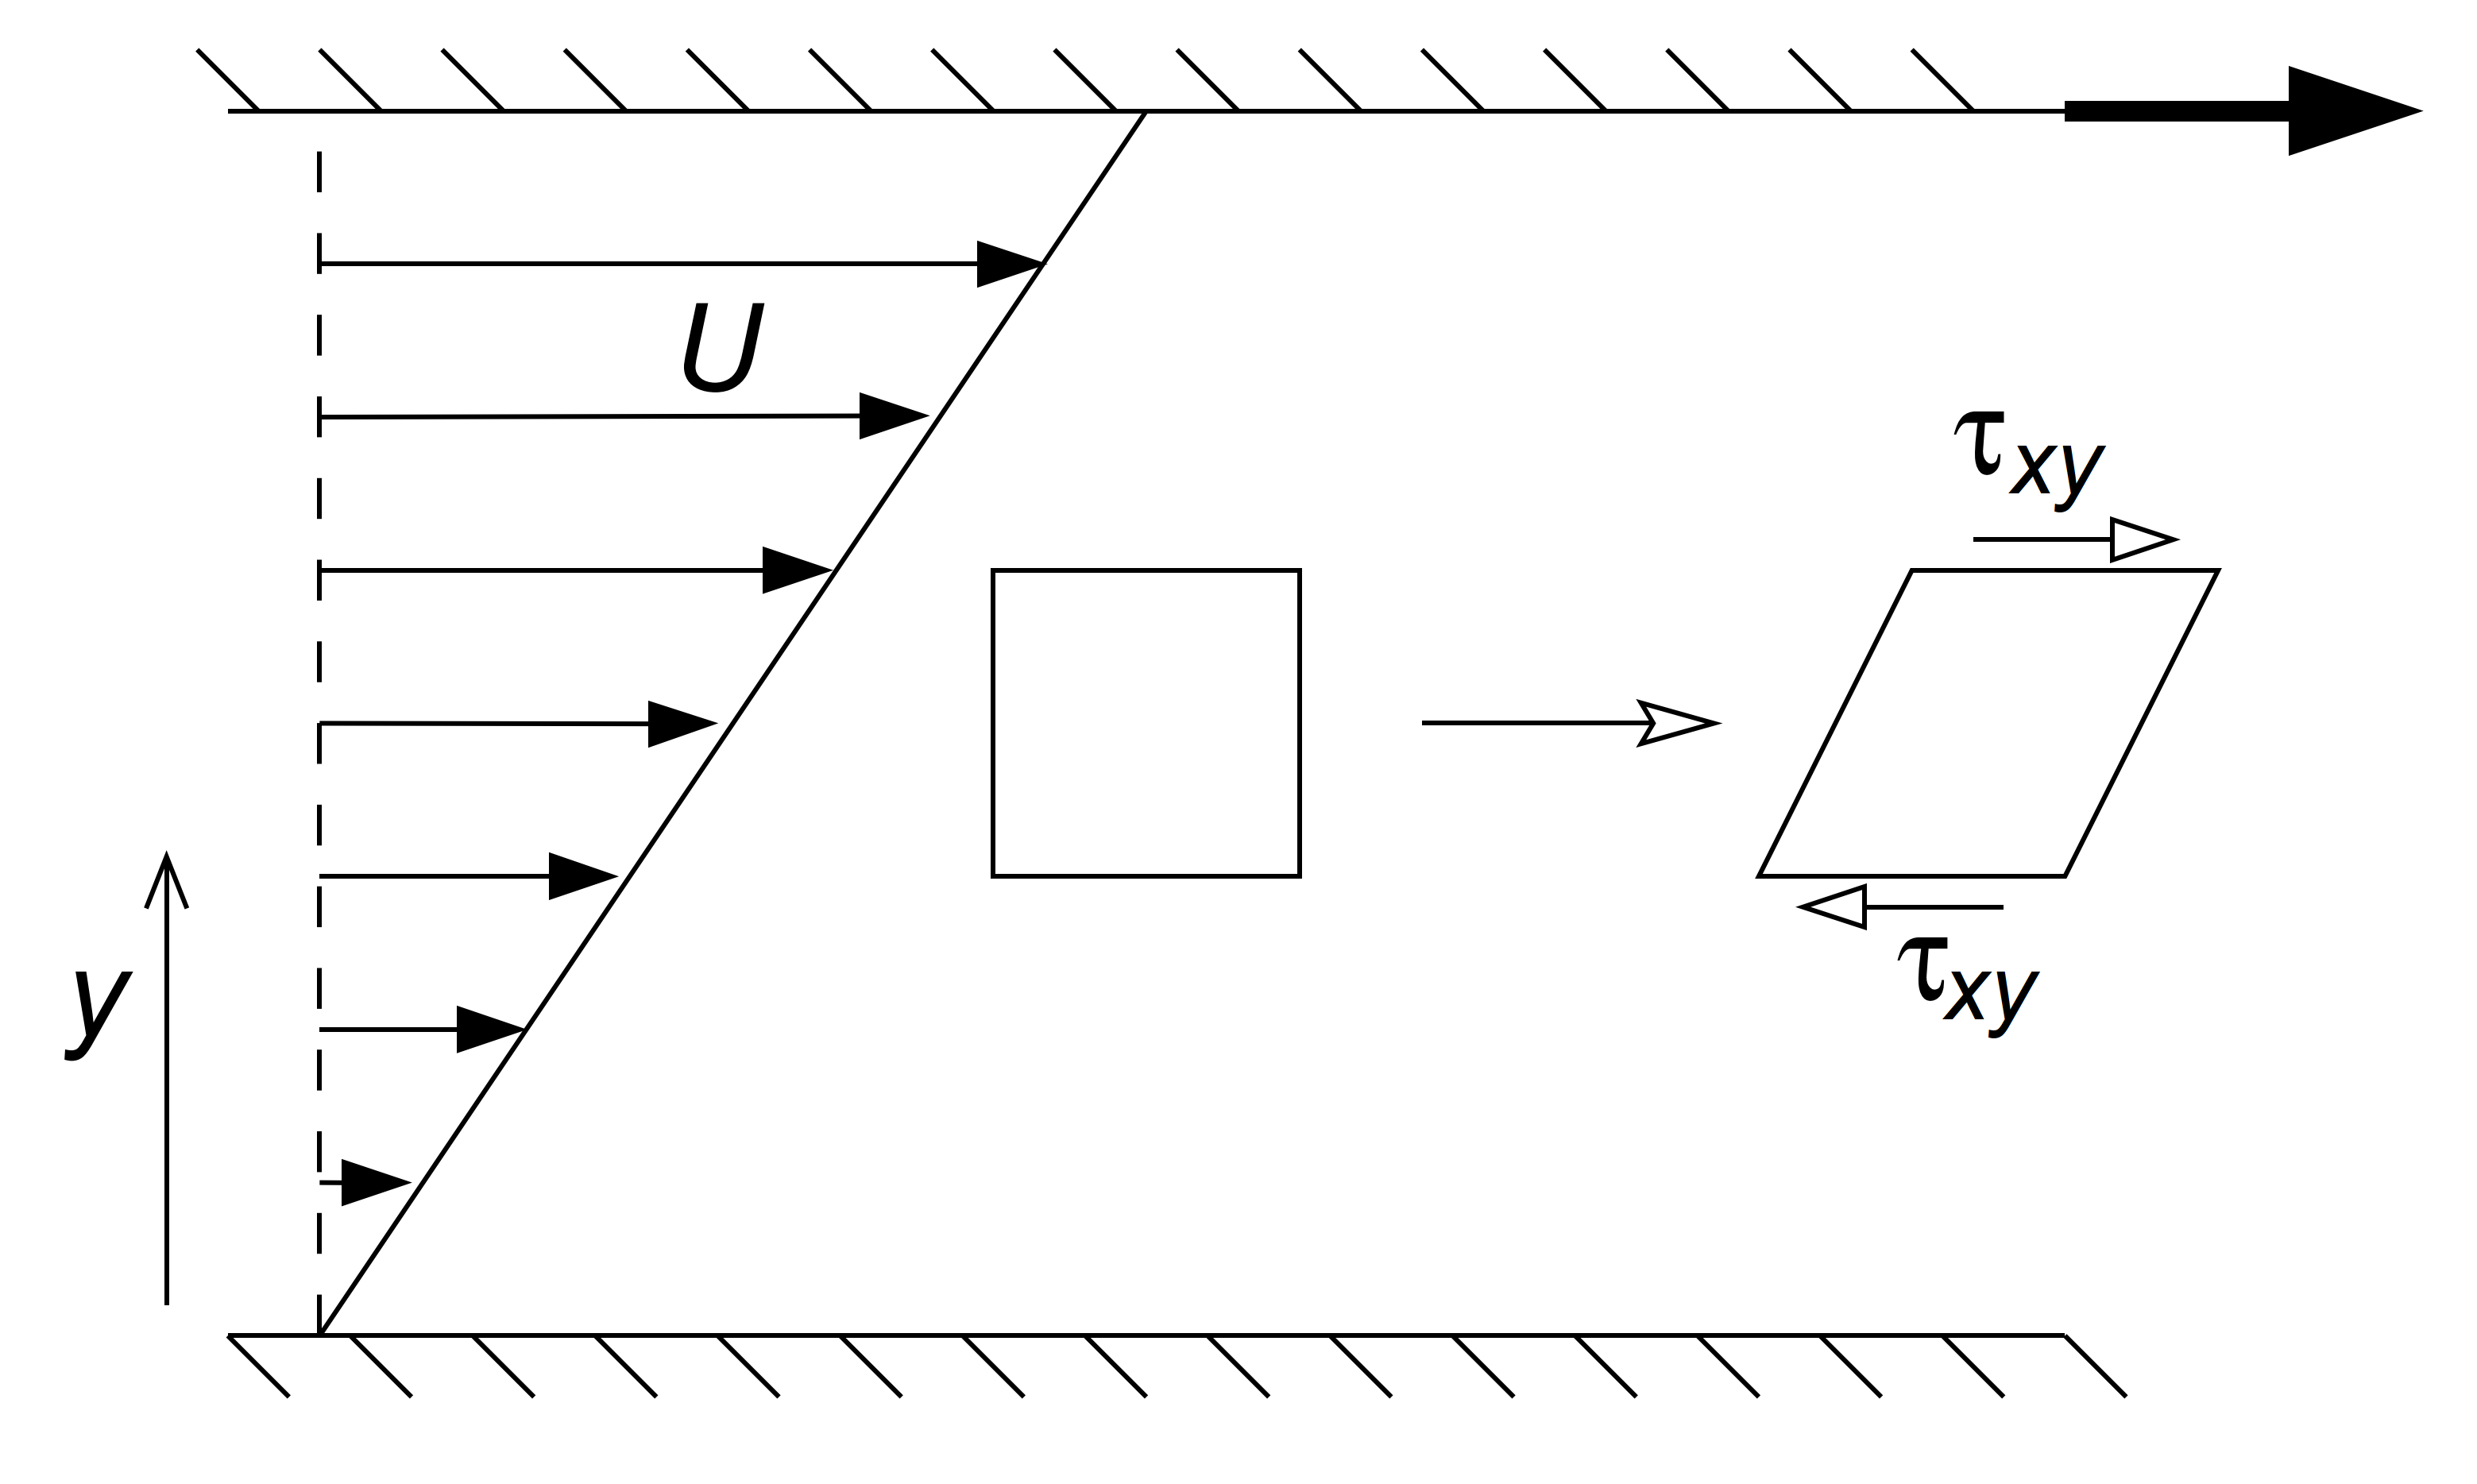
\includegraphics[scale = 0.1]{viscosity.PNG}
\end{figure}

The viscous shear stress is related to the velocity gradient along the perpendicular direction. Fluids follow this behaviour are referred as Newtonian fluids.

\begin{equation}
\tau_{xy} = -\mu \frac{\partial U}{\partial y}
\end{equation}
For Newtonian fluids these general stress-strain relations can be expressed as the viscous stresses being linearly related to the strain rates, with the constant of proportionality being the viscosity $\mu$.
\begin{equation}
\tau_{xx} = -2\mu \frac{\partial U}{\partial x} \textbf{\quad}   \tau_{yy} = -2\mu \frac{\partial V}{\partial y} \textbf{\quad} \tau_{xy} = -\mu( \frac{\partial U}{\partial y} + \frac{\partial V}{\partial x})
\end{equation}
Substitute this relation to the \ref{eq:momentum x}. 
\begin{align*}
\frac{\partial(\rho U)}{\partial t} + &\frac{\partial (\rho U^2)}{\partial x} + \frac{\partial (\rho UV)}{\partial y} +\frac{\partial (\rho UW)}{\partial z} = -\frac{\partial p}{\partial x} + \rho F_x \\
&+2\frac{\partial}{\partial x}\left[\mu \frac{\partial U}{\partial x}\right] + \frac{\partial}{\partial y}\left[ \mu \left(\frac{\partial U}{\partial y} + \frac{\partial V}{\partial x} \right) \right] + \frac{\partial}{\partial z}\left[ \mu \left(\frac{\partial U}{\partial z} + \frac{\partial W}{\partial x} \right) \right]
\label{eq:momentum x without tau}
\end{align*}

Similar equations exist for $y, z$ directions and put them in index form:

\begin{equation}
\frac{\partial \rho u_i}{\partial t} + \frac{\partial \rho u_i u_j}{\partial x_j} = -\frac{\partial p}{\partial x_i} + \frac{\partial }{\partial x_j}\left(\mu \frac{\partial u_i}{\partial x_j}\right) + \rho F_i
\end{equation}
Combine the mass and momentum conservation equations together are the Navier-Stokes equations. 
\begin{equation}
	\begin{cases}
    		\dfrac{\partial \rho}{\partial t} + \dfrac{\partial (\rho u_i)}{\partial x_i} = 0  \\
        \dfrac{\partial \rho u_i}{\partial t} + \dfrac{\partial \rho u_i u_j}{\partial x_j} = -\dfrac{\partial p}{\partial x_i} + \dfrac{\partial }{\partial x_j}\left(\mu \dfrac{\partial u_i}{\partial x_j}\right) + \rho F_i
    \end{cases}
\end{equation}

Instead of the above simplification, other way to proceed is decomposing the stress to normal and shear parts: 
\begin{equation}
\boldsymbol {\tau }=\zeta (\nabla \cdot \mathbf {u} )\mathbf {I} +\mu \left(\nabla \mathbf {u} +(\nabla \mathbf {u} )^{\mathrm {T} }-{\tfrac {2}{3}}(\nabla \cdot \mathbf {u} )\mathbf {I} \right)
\end{equation}

For a incompressible case, the density $\rho$ is a constant. The mass continuity equation can be simplified to: 

\begin{equation}
\frac{\partial u_i}{\partial x_i} = 0
\end{equation}

Further, if the viscosity is a constant, the diffusion can be simplified by taking $\mu$ outside the derivatives and combine the mass conservation condition. This form is quite commonly seen in texts.

\begin{equation}
\frac{\partial u_i}{\partial t} +  u_i \frac{\partial  u_j}{\partial x_j} = -\frac{1}{\rho} \frac{\partial p}{\partial x_i} + \mu\left( \frac{\partial^2 u_i }{\partial x_i x_j }\right) + \rho F_i
\end{equation}
The first term usually is referred as the time derivative term, the second term is the convection term, the laplacian term of the velocity is the diffusion term. The body force neglected.

\begin{equation}
\begin{cases}
   \dfrac{\partial \mathbf{u}}{\partial t} + \left(\mathbf{u} \cdot \nabla \right) \mathbf{u}  = -\dfrac{1}{\rho} \nabla p + \nu \nabla ^2 \mathbf{u}        \\
 \nabla \cdot \mathbf{u}  = 0
\end{cases}
\end{equation}

For incompressible case, the viscosity usually is replaced by kinematic viscosity as the above equations indicated.
$$
\nu = \frac{\mu}{\rho}
$$

The components of viscous stress tensor $\tau_{ij}$ in Navier-Stokes equations is defined as :
\begin{equation}
\tau_{ij} = 2\mu S_{ij} + \lambda \frac{\partial u_i}{\partial x_i} \delta_{ij}
\end{equation}

For the rotating frame reference introduced some interesting pseudo-forces into the equations through the material derivative term. Consider a stationary inertial frame of reference K, and a non-inertial frame of reference K', which is translating with velocity $\mathbf{U}(t)$ and rotating with angular velocity $\mathbf{\Omega}(t)$ with respect to the stationary frame. The Navier–Stokes equation observed from the non-inertial frame then becomes

\begin{equation}
\rho {\frac {D\mathbf {u} }{Dt}}=-\nabla \bar{p} +\mu \nabla^{2}\mathbf{u} +{\tfrac {1}{3}}\mu \nabla (\nabla \cdot \mathbf{u} )+\rho \mathbf{g} -\rho \left(2\mathbf{\Omega } \times \mathbf{u} +\mathbf{\Omega } \times (\mathbf{\Omega } \times \mathbf{x} )+{\frac {d\mathbf{U} }{dt}}+{\frac {d\mathbf{\Omega } }{dt}}\times \mathbf{x} \right)
\end{equation}
Here $\mathbf {x}$, $\mathbf {U}$ are measured in the non-inertial frame. The first term in the parenthesis represents Coriolis acceleration, the second term is due to centrifugal acceleration, the third is due to the linear acceleration of K' with respect to K and the fourth term is due to the angular acceleration of K' with respect to K.


\subsubsection{Energy Conservation}

First law of thermodynamics, the rate of change of energy (left hand side) is equal to the sum of rate of added heat (negative part of the right-hand side) and the rate of work done (positive part of right-hand side).

\begin{equation}
\rho \frac{D}{Dt}\left(e + \frac{1}{2}u_i u_i\right) = \rho F_i u_i - \frac{\partial}{\partial x_i}(pu_i)+\frac{\partial}{\partial x_i}(\tau_{ij}u_j) - \frac{\partial q}{\partial x_i}
\end{equation}
The internal energy change rate, equals the work rate contributed by the body force, the pressure surface work, viscous surface stress, heat flux.

The heat flux need to be related to the temperature gradients with Fouriers law.
\begin{equation}
q_i = -\kappa \frac{\partial T}{\partial x_i}
\end{equation}
where $\kappa = \kappa(T)$ is the thermal conductivity. This allows us to write the thermal energy equation as
Alternative form of the thermal energy equation can be derived using the definition of the enthalpy
\begin{equation}
h = e + \frac{p}{\rho}
\end{equation}

\noindent
[Rate of energy change in CV ] =  [Rate of net energy change in CV] + 

\noindent
[Work done by surface force acting on CV faces] + [Work done by sbody forces within CV]

\begin{align*}
 \frac{\partial}{\partial t}\left[ \rho\left( h +\frac{u_i u_i}{2}\right) \right] + \nabla \cdot \frac{\partial}{\partial t}\left[ \rho\left( e +\frac{u_i u_i}{2} \right) \right]\\
 = \rho \dot{q} &+ \frac{\partial}{\partial x}\left(k \frac{\partial T}{\partial x}\right) + \frac{\partial}{\partial y}\left(k \frac{\partial T}{\partial y}\right) + \frac{\partial}{\partial z}\left(k \frac{\partial T}{\partial z}\right)\\
 &- \frac{\partial(u_xp)}{\partial x} - \frac{\partial(u_xp)}{\partial y} - \frac{\partial(u_zp)}{\partial z} \\
 &+ \frac{\partial(u_x \tau_{xx})}{\partial x} + \frac{\partial(u_x \tau_{yx})}{\partial y} +\frac{\partial(u_x \tau_{zx})}{\partial z} \\
 &+ \frac{\partial(u_y \tau_{xy})}{\partial x} + \frac{\partial(u_y \tau_{yy})}{\partial y} +\frac{\partial(u_y \tau_{zy})}{\partial z} \\
 &+ \frac{\partial(u_z \tau_{xz})}{\partial x} + \frac{\partial(u_z \tau_{yz})}{\partial y} +\frac{\partial(u_z \tau_{zz})}{\partial z} \\
 &+ \rho F_i u_i
\end{align*}

\subsubsection{Transport equations}
The transport equation describes how a scalar quantity is transported in a space. Usually, it is applied to the transport of a scalar field (e.g. chemical concentration, material properties or temperature) inside an incompressible flow. From the mathematical point of view, the transport equation is also called the convection-diffusion equation, which is a first order PDE (partial differential equation). The convection-diffusion equation is the basis for the most common transportation models. The transport equation (or convection-diffusion equation) can be seen as the generalization of the continuity equation. While the continuity equation (extensively described in the article about incompressible flow) usually describes the conservation of mass, the convection-diffusion equation describes the continuity/conservation of any scalar field in any space. Let’s consider an infinitesimal portion of space $\Omega$ and its boundaries $\Gamma$. A conservation field around the volume should fulfil the following equations.
\begin{equation}
\frac{\partial}{\partial t}\int_\Omega \phi d\Omega =  -\int_\Gamma Fd\Gamma + \int_\Omega Q d \Omega
\end{equation}


A continuity equation (or conservation law) is an integral relation stating that the rate of change of some integrated property $\phi$  defined over a control volume $\Omega$  must be equal to what amount is lost or gained through the boundaries $\Gamma$ of the volume plus what is created or consumed by sources and sinks inside the volume. 
The numerical integration is then easily done by evaluate the volume integral and the surface integral at the finite cell center. The average value of the cell is stored at the centroid of the cell, the volume of the cell $\times$ the average value is then the integral. The surface integral follows the same way, surface area $\times$ the average surface value. 

A general form of this is: Time derivative ($d\phi/dt$) + Convection terms ($du_i\phi/dx_i$) = Diffusion terms ($d\phi^2 / dx_i$) + Source terms($S_i$). This can be $u_i, T$. Later the transport equation for turbulence related quantities, chemical concentration.... 


This is expressed by the following integral continuity equation:
\begin{equation}
\frac{\partial \phi}{\partial t} + \frac{\partial (u_i\phi)}{\partial x_i} = \frac{\partial}{\partial x_i}(\frac{\partial \phi}{\partial x_i}) + S_i
\end{equation}
where $u_i$ is the flow velocity of the fluid and $ s $ represents the sources and sinks in the flow, taking the sinks as positive. These equations can be directly solved by numerical method. This way is called DNS, direct numerical simulation. It is very accurate. However, since the turbulence is usually at very small scale, not practical for engineering application. 
\subsection{Turbulence}

\begin{figure}
\centering
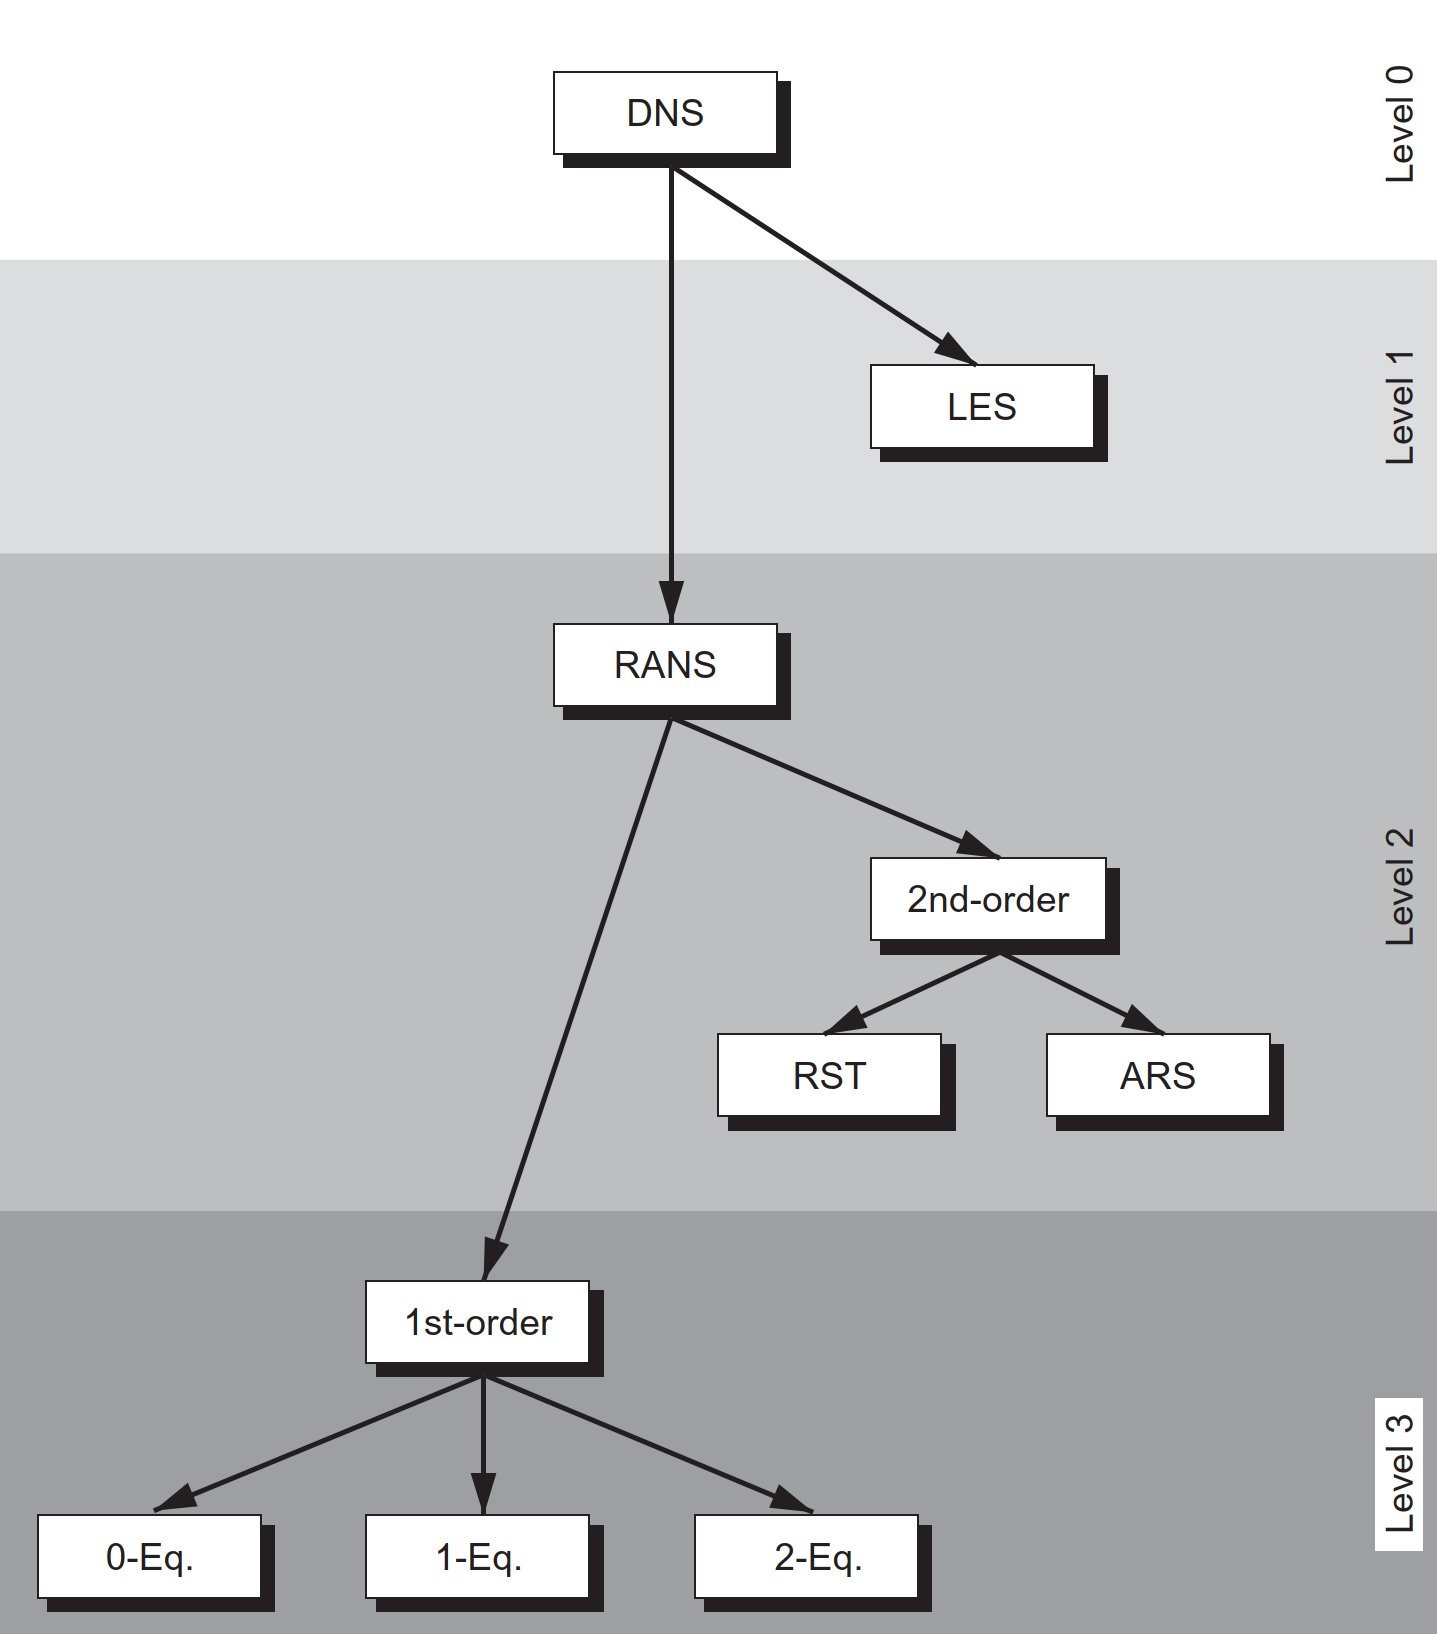
\includegraphics[scale=0.25]{turbulence models.PNG}
\caption{The hierarchy of turbulence models. DNS: direct numerical simulation, LES: large-eddy simulation, ARS: algebraic
Reynolds-stress models, RANS: Reynolds-averaged Navier-Stokes equations, 1st-order, first-order closure, RST: Reynolds.stress transport models}
\end{figure}


Swirls and circulations, randomness makes it very hard to predict. 


The average based method is the most commonly used. The Reynolds-Averaged Navier-Stokes (RANS) technique. Every parameter $u$ is divided to mean part $\bar{u}$ and fluctuating part $ u^\prime $, as $u = \bar{u} + u^\prime$ All other parameters $p,\ T$ can be divided like this to mean and fluctuating. Then Time averaging appropriate for stationary turbulence (statistically steady turbulence), Spatial averaging appropriate for homogeneous turbulence and Ensemble averaging—appropriate for general turbulence.

For all three approaches, the average of the fluctuating part is zero, that is, $\overline{v_i ^\prime}$ = 0.
However, it can be easily seen that $\overline{v_i ^\prime v_i ^\prime} \neq 0$. The same is true for $\overline{v_i ^\prime v_j ^\prime} \neq 0$, if both turbulent velocity components are correlated.

The model is coming from the averaged Reynolds stress tensor, $\bar{u_l ^\prime u_j ^\prime}$ is a symmetric tensor and contains 6 new unknown variables without adding new equations. How to solve the unconstrained equations is the main different between the models. The mostly used $k−\epsilon $ and $k−\omega $ models use the Boussinesq assumption to model the Reynolds stress tensor. The boussinesq assumption relates the Reynolds stress tensor to the velocity gradients and turbulent viscosity as the following. 

There are many variants such as one equation model and two equations models. Of the two equations model variants of the $k−\epsilon $ and the $k−\omega $ models are among others the most used.  The $ k $ is stand for turbulent kinetic energy, $ \epsilon $ is the turbulent dissipation, $\omega$ is the specific dissipation. The RANS models can be divides into different groups: Algebraic models; One equation model; Two equations models; Reynolds stress models. 

\begin{equation}
\begin{cases}
\frac{\partial \overline{u}_i}{\partial t} + \overline{u}_j \frac{\partial \overline{u}_i}{\partial x_j} = -\frac{1}{\rho}\frac{\partial \overline{p}}{\partial x_i} + \mu \nabla^2\overline{u}_i-\frac{\partial}{\partial x_j}(\overline{u_i ^\prime u_j ^\prime})\\
\frac{\partial \overline{u}_i}{\partial x_i} = 0
\end{cases}
\end{equation}
where the $u_i = \bar{u_i}$ is the average of the continuity equation also has been added. We find the Reynolds average equations

\begin{equation}
\overline{u_l ^\prime u_j ^\prime}=-\nu _T(\frac{\partial \bar u_i}{\partial x_j} 
 \frac{\partial \bar u_j}{\partial x_i})+\frac{2}{3}k\delta _{ij}=-2\nu _t s_{ij} +\frac{2}{3}k\delta _{ij}
\end{equation}

\begin{equation}
\frac{\partial}{\partial x_j}(\overline{u_i ^\prime u_j ^\prime})
 = \frac{\partial}{\partial x_j}
  \begin{bmatrix}
   \overline{(v_1 ^\prime)^2} & \overline{v_1 ^\prime v_2 ^\prime}  &  \overline{v_1 ^\prime v_3 ^\prime} \\
   \overline{v_2 ^\prime v_1 ^\prime} &  \overline{(v_2 ^\prime)^2} &   \overline{v_2 ^\prime v_3 ^\prime} \\
   \overline{v_3 ^\prime v_1 ^\prime} &  \overline{v_3 ^\prime v_2 ^\prime} & \overline{(v_3 ^\prime)^2}   
   \end{bmatrix}
\end{equation}

However, since $v_i ^\prime$ and $v_j ^\prime$ in the correlations can be interchanged, the Reynolds-stress 
tensor contains only six independent components. The sum of the normal stresses divided by density defines the turbulent kinetic energy, that is,
\begin{equation}
K = \frac{1}{2} \overline{v_i ^\prime v_i ^\prime	} = \frac{1}{2}\left[ \overline{(v_1 ^\prime)^2} + \overline{(v_2 ^\prime)^2} + \overline{(v_3 ^\prime)^2}  \right]
\end{equation}
As we can see here, the fundamental problem of turbulence modelling based on the Reynolds-averaged Navier-Stokes equations is to find six additional relations in order to close the NS.

The 


\part{OpenFOAM case setup}

\section{Numerical}
OpenFOAM applications are designed for use with unstructured meshes, offering up to second order accuracy, predominately using collocated variable arrangements. Most focus on the Finite Volume Method, for which the conservative form of the general scalar transport equation for the property $\phi$ takes the form:

\begin{equation}
\underbrace{\frac{\partial}{\partial t} (\rho\phi)}_{\mathrm{unsteady}} + \underbrace{\nabla \cdot (\rho \phi \textbf{u})}_{\mathrm{convection}} = \underbrace{\nabla \cdot (\Gamma \nabla \phi)}_{\mathrm{diffusion}} + \underbrace{S_{\phi}}_{\mathrm{source}}
\label{eq:transport equation}
\end{equation}


\begin{table}[hbp!]
\begin{tabular}{l l}
	unsteady: &   time dependent\\
	convection & velocity dependent\\
	diffusion & viscosity dependent \\
	source & heat, force...
\end{tabular}
\end{table}
The finite volume method requires the integration over a 3D-control volume, such that:
\begin{equation}
\int_V \frac{\partial}{\partial t} {(\rho \phi)} dV + \int_V \nabla \cdot \left(\rho \phi \textbf{u} \right) dV = \int_V \nabla \cdot \left(\Gamma \nabla \phi \right) dV + \int_V S_\phi dV 
\label{eq:intergal transport equation}
\end{equation}
or in a more compact way:

\begin{equation}
\textit{\textbf{A}}\textbf{x} = \textbf{b}
\end{equation}
where
\begin{table}[hbp!]
\begin{tabular}{l l}
	A: &   coefficient matrix\\
	x & vector of unknows dependent\\
	b & source vector
\end{tabular}
\end{table}

The discretisation process employs user selected schemes to build the A matrix and b vector, described in the following sections. Choice of schemes are set in the \textit{fvSchemes} dictionary.

OpenFOAM includes a wide range of solution and scheme controls, specified via dictionary files in the case system sub-directory. These are described by:

Numerical schemes: The treatment of each term in the system of equations is specified in the fvSchemes dictionary. This enables fine-grain control of e.g. temporal, gradient, divergence and interpolation schemes.

Linear equation solvers Solution methods: Case solution parameters are specified in the fvSolution dictionary. These include choice of linear equation solver per field variable, algorithm controls e.g. number of inner and outer iterations and under-relaxation.

Finite volume options: Additional run-time selectable physical modelling and general finite terms are prescribed in the fvOptions dictionary, targeting e.g. acoustics, heat transfer, momentum sources, multi-region coupling, linearised sources/sinks and many more.

\subsection{Schemes}

\subsection{Temporal schemes}

OpenFOAM includes a variety of schemes to integrate fields with respect to:

Time schemes

Time schemes define how a property is integrated as a function of time, i.e.
\begin{equation}
\frac{\partial}{\partial t}(\phi)
\end{equation}
Depending on the choice of schemes, field values at previous time steps are required, represented in the following as $\phi^0$ and $\phi^{00}$ for the old and older time levels. 

Usage 

Time schemes properties are input in the \textit{fvSchemes} file under the \textit{ddtSchemes} sub-directory using the syntax:

\begin{verbatim}
ddtSchemes
{
    default         none;
    ddt(Q)          <time scheme>;
}
\end{verbatim}
 
Available time schemes include
\begin{itemize}
\item Backward time scheme
\begin{equation}
\frac{\partial}{\partial t}(\phi) = \frac{1}{\Delta t}(\frac{3}{1}\phi - 2\phi^0 + \frac{1}{2} \phi^{00})
\end{equation}
Using implicit, second order accuracy, transient, boundedness not guaranteed, conditionally stable. 

Usage 

\begin{verbatim}
ddtSchemes
{
    default         backward;
    ddt(phi)        backward;
}
\end{verbatim}

\item Crank-Nicolson time scheme
Second order, Transient, Bounded, when using uniform time steps the schemes equate to: 
\begin{equation}
\frac{\partial}{\partial t} = \frac{\phi - \phi^{00}}{2\Delta t}
\end{equation}

Usage

The schemes is specified using: 

\begin{verbatim}
ddtSchemes
{
    default         CrankNicolson <coeff>;
    ddt(phi)        CrankNicolson <coeff>;
}
\end{verbatim}

The coefficient provides a blending between Euler and Crank-Nicolson schemes:

0: Euler
1: Crank-Nicolson
A value of 0.9 is a good compromise between accuracy and robustness

\item Euler implicit time scheme

Implicit, First order, Transient 
\begin{equation}
\frac{\partial}{\partial t} = \frac{\phi - \phi^0}{\Delta t}
\end{equation}

Usage

\begin{verbatim}
ddtSchemes
{
    default         Euler;
    ddt(phi)        Euler;
}
\end{verbatim}


\item Local Euler implicit/explicit time scheme
First order
Pseudo transient, designed for steady cases
Spatially varying, cell-based time scale set by specific Local Time Stepping (LTS) solvers

Usage

\begin{verbatim}
ddtSchemes
{
    default         localEuler;
    ddt(phi)        localEuler;
}
\end{verbatim}

\item Steady state time scheme
Steady state, set temporal derivative contributions to zero, 
\begin{equation}
\frac{\partial}{\partial t} = 0
\end{equation}
\end{itemize}

\subsection{Spatial schemes}

At their core, spatial schemes rely heavily on \textit{interpolation schemes} to transform cell-bases qualities to cell faces, in combination with \textbf{Gauss Theorem} to convert volume integrals to surface integrals.

\begin{itemize}
\item Gradient Schemes
\item Divergence schemes
\item Laplacian schemes
\item Surface-normal gradient schemes
\end{itemize}

\subsection{Wall distance calculation method}

Distance to the nearest wall is required, e.g. for a number of turbulence models. Several calculation methods are available:
\begin{itemize}
\item Mesh-wave wall distance
\item Poisson wall distance 
\end{itemize}

\subsection{Solutions}

After using different schemes to build the equation systems. The next step is to chose a technic to solve the linear equations, the matrix sytem. 
\begin{equation}
x = A^{-1}b
\end{equation}
where the inverse of the diagonal matrix is simply:
\begin{equation}
A^{-1} = \frac{1}{diag(A)}
\end{equation}
This is available as the diagonalSolver. More tyically the matrix cannot be inverted easily and the system is solved using iterative methods, as discribed in the following sections. 

\subsection{Solvers}

\begin{itemize}
\item Smooth solvers
\item Conjugate gradient solvers
\item Multigrid solvers
\end{itemize}

\subsection{Solver control}
\begin{itemize}
\item Under relaxation
\item Residuals
\item Case termination
\end{itemize}

Common usage
minIter: minimum number of solver iterations
maxIter: maximum number of solver iterations
nSweeps: number of solver iterations between checks for solver convergence
Implementation details
Matrix structure
Matrix coefficients are stored in upper-triangular order

neighbour cell index always higher than owner cell index across a face
when looping over cell faces, the face index increases with increasing cell index
for the 1-D case, if cell index 0 is at the boundary, this equates to a monotonic increase in cell numbers, i.e. defines a continuous sweep across the 1-D region
used in Gauss-Seidel method


\section{boundary condition}

Boundary conditions are extremely important. Indeed, they cause the most common errors.
OpenFOAM uses similar set-up as other solvers.
\begin{itemize}
    \item At the inlet (flow inlet) to the computational domain total pressure and total temperature are set. The rest of variables are reconstructed.
    \item At the outlet the static pressure is set.
    \item At the rigid walls velocity is set to zero.
    \item Multiple Reference Frame (MRF) is used for rotational components.
    \item For steady-state computations the initial conditions have no influence to the results.
    \item For steady-state computations the initial conditions just help to make the case run.
\end{itemize}

The main variables to be set are following:

p: static pressure p

U: velocity vector U

T: static temperature

k: turbulent kinetic energy k

$\omega$: specific turbulence dissipation 

$\epsilon$ specific turbulence dissipation

The initial and boundary conditions for all variables are set in files located in directories named by numbers. Typically directory 0 is recommended to start a simulation from. 

Initial conditions are set in parameter internalField putting the values into the cell centres. 

At boundaries, initial conditions are set individually by parameter value.

Following table shows recommended model of boundary conditions for computed variables:


\begin{landscape}
\begin{table}[h!]
    \centering
\begin{tabular}{cccccc}

\hline
boundaty type & p & U  & T & k & $\omega$ / $\epsilon$\\  
\hline
   	 	STATOR:	 \\
   	 	\hline
inlet &	totalPressure &	\makecell{pressureDirected\\InletVelocity} &	totalTemperature &	\makecell{turbulentIntensity\\KineticEnergyInlet} &	fixedValue   \\
volute\_wall &	zeroGradient &	fixexValue &	\makecell{compressible::\\turbulentTemperature\\CoupledBaffeMixed} &	\makecell{compressible::\\kqRWallFunction}	 & \makecell{compressible::\\omegaWallFunction}\\
ring* &	mixingPlane &	inletOutlet &	inletOutlet &	 inletOutlet &	inletOutlet\\
\hline	 	 	 	  
 	 	ROTOR	 	 	 \\
 	 	\hline
outlet &	fixedMeanValue &	inletOutlet &	inletOutlet	 & inletOutlet &	inletOutlet \\
outlet wall &	zeroGradient &	fixedValue	 & \makecell{compressible::\\turbulentTemperature\\CoupledBaffeMixed}	 & \makecell{compressible::\\kqRWallFunction} &	\makecell{compressible::\\omegaWallFunction} \\
wheel wall &	zeroGradient &	fixexValue &	zeroGradient	 & \makecell{compressible::\\kqRWallFunction} & 	\makecell{compressible::\\omegaWallFunction} \\
ring* &	zeroGradient &	mixingPlaneVelocity &	mixingPlane &	mixingPlane &	mixingPlane \\
\hline	 	 	 	 	  
 	 	SOLID:	 	 	 \\
 	 	\hline
rotor inner wall &	x &	x &	\makecell{compressible::\\turbulentTemperature\\CoupledBaffeMixed} &	x &	x \\
stator inner wall &	x &	x &	\makecell{compressible::\\turbulentTemperature\\CoupledBaffeMixed} &	x &	x \\
outer wall &	x &	x &	zeroGradient &	x &	x \\

  \hline

\end{tabular}
    \caption{Boundary condition recommondation$^*$}
    \label{tab:CFD-support recomm}
\end{table}

$^*$: taken from: 
\url{https://www.cfdsupport.com/Turbomachinery-CFD-manual/node283.html\#13201}
\end{landscape}






The shortcuts from the above table have following meaning:
\begin{itemize}
    \item tP - totalPressure constant, e.g. 250 000 Pa, gamma = 1.2853 [-] is specific heat ratio
    \item pDIV - pressureDirectedInletVelocity, velocity is computed from difference between total and static pressure, inletDirection is velocity vector to be specified
    \item tT - totalTemperature, constant, e.g. 1050 K, gamma= 1.2853 [-] is specific heat ratio
    \item tIKEI - turbulentIntensityKineticEnergyInlet, intensity = 0.02, corresponds to turbulence intensity 2%
    \item fV - fixedValue, e.g. velocity at the wall (0 0 0), or omega at inlet
    \item fMV - fixedMeanValue, is the same as fixed value, e.g. for pressure, but certain freedom is allowed to keep the variable average equal to meanValue
    \item zG - zeroGradient, the flux of the variable is zero in direction perpendicular to the surface
    \item TWF - compressible::turbulentTemperatureCoupledBaffleMixed special boundary condition for temperature enabling heat transfer from other regions
    \item kWF - compressible::kqRWallFunction is a standard wall function for k for compressible flow
    \item oWF - compressible::omegaWallFunction is a standard wall function for omega for compressible flow
    \item mPV - mixingPlaneVelocity, averaged velocity is mapped from neighbour patch
    \item mP - mixingPlane, averaged variable is mapped from neighbour patch
    \item iO - inletOutlet is by default zeroGradient, but changes to fixedValue when velocity vector direction points inside the computational domain (backward flow)
\end{itemize}


Another recommended boundary conditions for each vairable (depending on the selected turbulence model) at each boundary type. Note the variations for Wall BCs for a High Reynolds model(y+ 30-100), and a Low Reynolds model(y+ 1).


\newgeometry{left=1cm,right=1cm,top=1cm,bottom=1cm}
\begin{landscape}


\begin{table}[h!]
    \centering
\begin{tabular}{ccccccc}
\hline
  & inlet & outlet  & farfield & stationary walls & moving walls & rotating walls\\  
\hline
p &	\textbf{zeroGradient} &	\textbf{fixedValue 0 }&	\textbf{outletInlet 0} &	\textbf{zeroGradient} &	\textbf{zeroGradient}  & \textbf{zeroGradient}\\

U &	\makecell{\textbf{surfaceNormalFV} \\ negative value for \\ entry velocity}  &	\makecell{\textbf{zeroGradient} \\ \textbf{inletOutlet}}  & \makecell{\textbf{inletOutlet} \\ free stream velocity} & \makecell{\textbf{fixedValue 0}}	 & \makecell{\textbf{fixedValue}\\ velocity of the wall}  & \makecell{\textbf{rotatingWallVelocity} \\rotational \\velocity of the wall}\\

k &	\makecell{\textbf{fixedValue} \\ k = $(3/2)*(UI)^2$\\U:free stream velocity \\ I: Turbulent intensity} &	\makecell{\textbf{zeroGradient} \\ \textbf{inletOutlet}} & \makecell{ \textbf{inletOutlet} \\ k = $(3/2)*(UI)^2$\\U:free stream velocity \\ I: Turbulent intensity} & \makecell{\textbf{kqRWallFunction}\\(for y+ 30 to 100)\\\textbf{fixedValue 0} \\ (for y+ 1)}  & \makecell{\textbf{kqRWallFunction}\\(for y+ 30 to 100)\\\textbf{fixedValue 0} \\ (for y+ 1)} & \makecell{\textbf{kqRWallFunction}\\(for y+ 30 to 100)\\\textbf{fixedValue 0} \\ (for y+ 1)} \\

epsilon &\makecell{\textbf{fixedValue} \\ $\epsilon=0.09*k*\omega$} &	\makecell{\textbf{zeroGradient} \\ \textbf{inletOutlet}} &\makecell{ \textbf{inletOutlet} \\  $\epsilon=0.09*k*\omega$}	 & \makecell{\textbf{epsilonWallFunction} \\ (for y+ 30 to 100) \\ fixedValue $10^{-12}$ \\ (for y+ 1) }&	\makecell{\textbf{epsilonWallFunction} \\ (for y+ 30 to 100) \\ fixedValue $10^{-12}$ \\ (for y+ 1) } & \makecell{\textbf{epsilonWallFunction} \\ (for y+ 30 to 100) \\ fixedValue $10^{-12}$ \\ (for y+ 1) } \\

omega & 	\makecell{\textbf{fixedValue} \\ $\omega = \rho*\frac{k}{\mu}*(\frac{\mu_t}{\mu})^{-1}$\\ $\rho$:Density \\ k:Turbulence \\ kinetic energy \\ $\mu$: viscosity \\ $\mu_t$:turbulent viscosity} &	\makecell{\textbf{zeroGradient} \\ \textbf{inletOutlet}}	 & \makecell{\textbf{inletOutlet} \\ $\omega = \rho*\frac{k}{\mu}*(\frac{\mu_t}{\mu})^{-1}$\\ $\rho$:Density \\ k:Turbulence kinetic energy \\ $\mu$: viscosity \\ $\mu_t$:turbulent viscosity}	 &  \textbf{omegaWallFunction} &	\textbf{omegaWallFunction}  & \textbf{omegaWallFunction}\\

nutTilda &	\makecell{\textbf{fixedValue} \\ nuTilda = $\sqrt{3/2}*U*I*L$ \\ U:free stream velocity \\ I:turbulent intensity \\L:length scale} &	\makecell{\textbf{zeroGradient} \\ \textbf{inletOutlet}} & \makecell{\textbf{inletOutlet} \\ nuTilda = $\sqrt{3/2}*U*I*L$ \\ U:free stream velocity \\ I:turbulent intensity \\L:length scale}	 & \makecell{\textbf{zeroGradient} \\ (for y+ 30 to 100) \\ \textbf{fixexValue 0} \\ (for y+ 1)} & 	\makecell{\textbf{zeroGradient} \\ (for y+ 30 to 100) \\ \textbf{fixexValue 0} \\ (for y+ 1)} & \makecell{\textbf{zeroGradient} \\ (for y+ 30 to 100) \\ \textbf{fixexValue 0} \\ (for y+ 1)}  \\

nut & \textbf{calculated} &	\textbf{calculated} & \textbf{calculated}  &	\makecell{\textbf{nutkWallFunction} \\ (for y+ 30 to 100) \\ \textbf{nutUSpalding}\\\textbf{WallFunction} \\ (for y+ 1)} & \makecell{\textbf{nutkWallFunction} \\ (for y+ 30 to 100) \\ \textbf{nutUSpalding}\\\textbf{WallFunction} \\ (for y+ 1)} & \makecell{\textbf{nutkWallFunction} \\ (for y+ 30 to 100) \\ \textbf{nutUSpalding}\\\textbf{WallFunction} \\ (for y+ 1)}\\
\end{tabular}
    \caption{Boundary condition recommondation$^*$}
    \label{tab:ANSA recomm}
\end{table}
$^*$: taken from: 
ANSA for CFD Brief User's Guide. v19.1.2

\end{landscape}
\restoregeometry

\begin{landscape}
\begin{table}[h!]
    \centering
\begin{tabular}{cccccccccccc}

\hline
solver & transient & compressible  & turbulence & \makecell{heat\\transfer} & buoyancy & combustion & \makecell{multi\\phase} & particles& dynamicMesh & \makecell{multi\\region} & fvOptions\\  
\hline
boundaryFoam \\
\hline
buoyantPimpleFoam & $\surd$ & $\surd$ & $\surd$ & $\surd$ & $\surd$ & & & & & & $\surd$  \\
\hline
buoyantSImpleFoam & & & $\surd$ & $\surd$ & $\surd$ & $\surd$ & & & & & $\surd$ \\
\hline
chemFoam & $\surd$ & & & $\surd$ & & $\surd$ & & & & & \\
\hline
chtMultiRegionFoam & $\surd$ & $\surd$ & $\surd$ & $\surd$ & $\surd$ & & & & & $\surd$ & $\surd$ \\
\hline
coldEngineFoam & $\surd$ & $\surd$ & $\surd$ & $\surd$ & & $\surd$ & & & $\surd$ & & $\surd$ \\
\hline
engineFoam & $\surd$ & $\surd$ & $\surd$ & $\surd$ & & $\surd$ & & & $\surd$ & & $\surd$ \\
\hline
fireFoam & $\surd$ & $\surd$ & $\surd$ & $\surd$ & $\surd$ & $\surd$ & & & & $\surd$ & $\surd$ \\
\hline
icoFoam & $\surd$ & & & & & & & & & & \\
\hline
interFoam & $\surd$ & & $\surd$ & & & & $\surd$ & & $\surd$ & & $\surd$ \\
\hline
laplacianFoam & $\surd$ & & & & & & & & & & $\surd$ \\
\hline
pimpleFoam & $\surd$ & & $\surd$ & & & & & & $\surd$ & & $\surd$ \\
\hline
pisoFoam & $\surd$ & & $\surd$ & & & & & & & & $\surd$ \\
\hline
potensialFoam \\
\hline
reactingFoam & $\surd$ & $\surd$ & $\surd$ & $\surd$ & & $\surd$ & & & & & $\surd$ \\
\hline
reactingParcelFoam & $\surd$ & $\surd$ & $\surd$ & $\surd$ & $\surd$ & $\surd$ & & $\surd$ & & & $\surd$ \\
\hline
rhoCentralFoam & $\surd$ & $\surd$ & $\surd$ & $\surd$ & & & & & &  & \\
\hline
rhoPimpleFoam & $\surd$ & $\surd$ & $\surd$ & $\surd$ & & & & & $\surd$ & & $\surd$ \\
\hline
rhoSimpleFoam & & $\surd$ & $\surd$ & $\surd$ & & & & & & &  $\surd$\\
\hline
scalarTransportFoam & $\surd$ & & & & & & & & & & \\
\hline
simpleFoam & & & & & & & & &  & & $\surd$ \\	
\hline
spratFoam & $\surd$ & $\surd$ & $\surd$ & $\surd$ & $\surd$ & $\surd$& & $\surd$ & & & $\surd$ \\
\hline
XiFoam & $\surd$ & $\surd$ & $\surd$ & $\surd$ & & $\surd$ & & & & & $\surd$\\
\hline
\end{tabular}
    \caption{application solver capability matrix$^*$}
    \label{tab:solver compatibility}
\end{table}
$^*$: taken from: 
\url{https://www.openfoam.com/documentation/guides/latest/doc/openfoam-guide-applications-solvers.html#sec-applications-solvers-capability-matrix}

\end{landscape}



\section{Conclusion}
``I always thought something was fundamentally wrong with the universe'' \citep{adams1995hitchhiker}

\begin{figure}[h!]
\centering
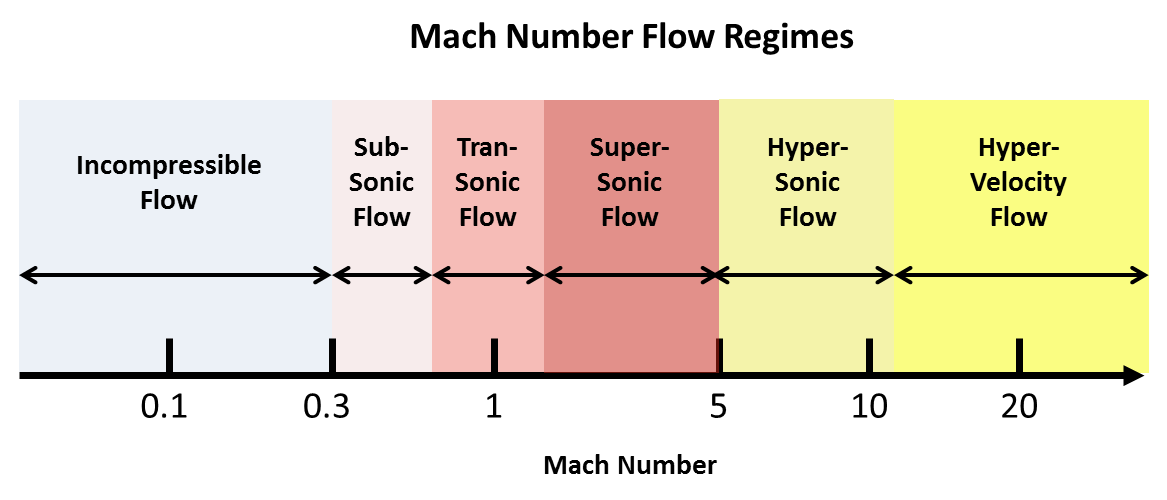
\includegraphics[scale=0.4]{compressible.png} 
\caption{compressible or incompressible dependence of Mach number.}
\label{fig:universe}
\end{figure}

\appendix
\section{Appendix}
Some important mathematics refreshments: 


\subsection{Gradient} 
$\nabla$,  For 1-dimensional domain, it is a standard derivative defined in calculus. 
For multi-dimensional domain, it may denote gradient, divergence, curl field. 
If $\nabla$ is applied to a scalar function, $f(x, y, z)$, it is the direction vector of the scalar function, stand for the local steepest slope.

\begin{equation}
grad \, f = \nabla f = \frac{\partial f}{\partial x} \vec e_1+\frac{\partial f}{\partial y} \vec e_2 +\frac{\partial f}{\partial z}\vec e_3 \quad or \quad \left( \frac{\partial f}{\partial x},\frac{\partial f}{\partial y},\frac{\partial f}{\partial z} \right)
\end{equation}

\subsection{Divergence} 
if the $\nabla$ is applied to a vector, it is the dot product of $\nabla$ with the vector $\nabla \cdot \vec{v}$ defined as: 

\begin{equation}
Div\, \vec v=\nabla \cdot \vec v = \frac{\partial v_x}{\partial x} +  \frac{\partial v_y}{\partial y}+\frac{\partial v_z}{\partial z}
\end{equation}

Divergence is a scalar function. It is the intensity of the converge flux toward or repel from a point. 

\subsection{Curl} 
$\nabla \times \vec{v}$ is the curl of a vector. It is a measure of the rotation of the vector field at the point. 

\begin{equation}
curl \, \vec v=\nabla \times \vec v=(\frac{\partial \vec v_z}{\partial y} - \frac{\partial \vec v_y}{\partial z})\vec e_x+(\frac{\partial \vec v_x}{\partial z} - \frac{\partial \vec v_z}{\partial x})\vec e_y+(\frac{\partial \vec v_y}{\partial x} - \frac{\partial \vec v_x}{\partial y})\vec e_z
\end{equation}

The result is refered as vorticity, If a cubic is thrown into a river, it rotates while if it flows, then there is vorticity in the river. 

\subsection{Laplacian} 
$\Delta$. It is a measure of the source. If there is no heat source inside a closed smooth surface, the Laplacian of heat flux on the closed surface should be zero. 
where: $\Delta q = 0$. 

\begin{equation}
\Delta f= \nabla \cdot \nabla f = \nabla ^2 f = \sum \frac{\partial ^2 f}{\partial x_i ^2} = \frac{\partial ^2 f}{\partial x^2}+\frac{\partial ^2 f}{\partial y^2}+\frac{\partial ^2 f}{\partial z^2}
\end{equation}

Description the diffusion: if there is no source in closed smooth surface, the Laplacian is zero, such as steady state heat transfer equation. 

\subsection{Gauss Theorem}
Gauss Theorem is also refereed as divergence theorem. It connects the volume integral to the closed surface integral.
If \textbf{u} is a continuously differentiable vector field defined on a neighborhood of V, then we have:

\begin{equation}
\int_V(\nabla \mathbf{u}) dV = \int_S(\mathbf{n} \cdot \mathbf{u}) dS 
\end{equation}

The left side is a volume integral over the volume V, the right side is the surface integral over the boundary of the volume V. The closed manifold $\partial V$ is quite generally the boundary of V oriented by outward-pointing normals, and n is the outward pointing unit normal field of the boundary $\partial V$. (dS may be used as a shorthand for ndS.) The symbol within the two integrals stresses once more that $\partial V$ is a closed surface. In terms of the intuitive description above, the left-hand side of the equation represents the total of the sources in the volume V, and the right-hand side represents the total flow across the boundary S.

In the physical theory of diffusion, the Laplace operator (via Laplace's equation) arises naturally in the mathematical description of equilibrium. Specifically, if u is the density at equilibrium of some quantity such as a chemical concentration, then the net flux of u through the boundary of any smooth region V is zero, provided there is no source or sink within V:

\begin{equation}
\int_{\partial V} \nabla u \cdot \mathbf {n} dS = 0
\end{equation}

where \textbf{u} is the outward unit normal to the boundary of V. By divergence theorem. 

\begin{equation}
\int_{V}  \text{div} \nabla u dV = \int_{\partial V} \nabla \cdot \textbf{u} dS = 0
\end{equation}

Since this holds for all smooth regions V, it can be shown that this implies

\begin{equation}
\text{div} \nabla u = \Delta u = 0
\end{equation}

The left-hand side of this equation is the Laplace operator. The Laplace operator itself has a physical interpretation for non-equilibrium diffusion as the extent to which a point represents a source or sink of chemical concentration, in a sense made precise by the diffusion equation.

Also known as diffusion, the Laplace operator (via Laplace's equation) arises naturally in the mathematical description of equilibrium.Specifically, if u is the density at equilibrium of some quantity such as a chemical concentration, then the net flux of u through the boundary of any smooth region V is zero, provided there is no source or sink within V.

\subsection{Material derivative}
In continuum mechanics, the material derivative describes the time rate of change of some physical quantity (like heat or momentum) of a material element that is subjected to a space-and-time-dependent macroscopic velocity field. The material derivative can serve as a link between Eulerian and Lagrangian descriptions of continuum deformation.

For example, in fluid dynamics, the velocity field is the flow velocity, and the quantity of interest might be the temperature of the fluid. In which case, the material derivative then describes the temperature change of a certain fluid parcel with time, as it flows along its pathline (trajectory).
\begin{equation}
\frac{D\phi}{Dt} = \frac{\partial \phi}{\partial t} + \frac{\partial (\phi u_i)}{\partial x_i}
\end{equation}
The first term is the change of $\phi$ over time, local part. The second term is the change due to the space variation. convection part.  

\subsection{Reynold transportation theorem}
In fact, it is a material derivative to a integral. Enable to evaluate the integral derivation of a time dependent function over a time with varies controlled volume. 
\begin{equation}
\frac{D}{Dt}\int_{V(t)} T_{ij} dV = \int _{V(t)} \left[ \frac{\partial T_{ij}}{\partial t} + \frac{\partial }{\partial x_k} \left( u_k T_{ij} \right) \right] dV
\end{equation}


\part{Visualization}

\section{VTK}

The VTK pipeline
The key to using VTK is to construct a pipeline. Most applications will go through similar stages when creating their pipeline. In approximately 4 general steps these are:
\begin{itemize}
\item Reading data: A visualisation needs data to visualise!

\item Filtering and processing data: Once data is read into the pipeline it often needs further processing and manipulation before it can be packaged into an actor.

\item  Creating actors from that data and assembling them in a scene: Data and geometry are packaged into an actor (don’t worry, more on this will follow below).

\item  Assembling pieces of geometry into a final render: The actors described above are positioned and an interactive 3D environment is rendered.
\end{itemize}

You can probably tell by now that VTK uses the metaphor of a theatre/film set when describing the rendering environment. The goal of the early stages of a VTK pipeline is to read data including information about the geometry of a model and  package it into an actor. An actor is an instance of an object that includes all of the information necessary for rendering (how to do this will be explained below). These actors will be arranged in a scene by you and rendered. The scene created by VTK is is interactive. The user will be able to move around and rotate the objects. It is possible, if programmed into the visualisation, to cut, move, and otherwise manipulate these actors to get at precisely the part of the geometry that is of most interest to the user.

\begin{figure}
\centering
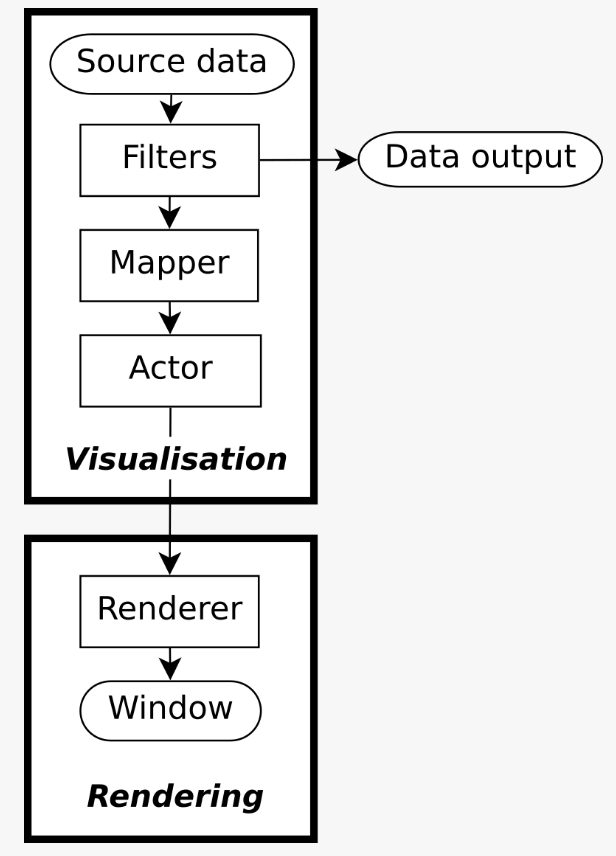
\includegraphics[scale=0.6]{VTK pipe line.PNG}
\caption{The pipe line of the VTK visualization}
\label{fig:VTK pipe line}
\end{figure}


Creating a mapper is an intermediate step in the visualisation pipeline. It takes data and eeds into an actor. Its role is to map data into graphics primitives. For polygon meshes this is more straightforward than other types of data. It also includes making settings about how data is converted to colours (see lookup tables below), or whether to use cell data or node data to colour a model. The actor is concerned with how the model fits into the scene. As a result parameters that can be set from within the actor often concern texturing, lighting, positioning etc. of the object within the scene.

The final steps to complete the visualisation are the following.
\begin{verbatim}
window = vtk.vtkRenderWindow()
# Sets the pixel width, length of the window.
window.SetSize(500, 500)

interactor = vtk.vtkRenderWindowInteractor()
interactor.SetRenderWindow(window)

renderer = vtk.vtkRenderer()
window.AddRenderer(renderer)

renderer.AddActor(actor)
# Setting the background to blue.
renderer.SetBackground(0.1, 0.1, 0.4)

window.Render()
interactor.Start()
\end{verbatim}

A lookup table for polygon data is created using lut = vtk.vtkPolyDataMapper(). The lookup table is associated with a model through the mapper object. The method .SetLookupTable(lut) connects the lookup table lut to the mapper. Further, the method .SetUseLookupTableScalarRange(True) needs to be called on the mapper. This causes the mapper to use the same range as that used by the lookup table. Not using this method will cause the mapper to override the range set in the lookup table which is probably not what you want.

\bibliographystyle{plain}
\bibliography{references}
\end{document}
